\documentclass[%
    reprint,
   %superscriptaddress,
   %groupedaddress,
   %unsortedaddress,
   %runinaddress,
   %frontmatterverbose, 
   %preprint,
   %showpacs,preprintnumbers,
   %nofootinbib,
   %nobibnotes,
   %bibnotes,
    amsmath,amssymb,
    aps,
   %pra,
   %prb,
   %rmp,
   %prstab,
   %prstper,
   %floatfix,
   ]{revtex4-1}
   
   \usepackage{graphicx}% Include figure files
   \usepackage{dcolumn}% Align table columns on decimal point
   \usepackage{bm}% bold math
   \documentclass{article}
   \usepackage[utf8]{inputenc}
   \usepackage{stmaryrd}
   \usepackage{amsmath}
   \usepackage{float}
   %\usepackage{hyperref}% add hypertext capabilities
   %\usepackage[mathlines]{lineno}% Enable numbering of text and display math
   %\linenumbers\relax % Commence numbering lines
   
   %\usepackage[showframe,%Uncomment any one of the following lines to test 
   %%scale=0.7, marginratio={1:1, 2:3}, ignoreall,% default settings
   %%text={7in,10in},centering,
   %%margin=1.5in,
   %%total={6.5in,8.75in}, top=1.2in, left=0.9in, includefoot,
   %%height=10in,a5paper,hmargin={3cm,0.8in},
   %]{geometry}
   
   \begin{document}
   
   \title{New LSB-pair methods to reduce distortion of watermarking image}% Force line breaks with \\
   \thanks{A footnote to the article title}%
   
   \author{Shuyan Hu}
    \altaffiliation[Also at ]{School of Engineering, the University of Melbourne.}
    \email{hushuyan88@gmail.com}
   % \author{Second Author}%
   %  \email{Second.Author@institution.edu}
   % \affiliation{%
   %  Authors' institution and/or address\\
   %  This line break forced with \textbackslash\textbackslash
   % }%
   
   % \collaboration{MUSO Collaboration}%\noaffiliation
   
   \date{\today}% It is always \today, today,
                %  but any date may be explicitly specified
   
   
   \begin{abstract}
   Digital watermarking is a technology which can embed information to digital image, video and audio. Digital watermarking can be done by Least Significant Bit (LSB) which is a method of replacing pixel least bit with message bits. This modification can disturb carrier image pixel distribution and increase image distortion irresistibly which can raise the risk of being detected. This thesis proposes a new method named LSB-pair aiming and its advanced methods to reduce watermarked image distortion. These methods are based on LSB replacement, hence, they can be considered as variations of LSB replacement. On our experiment, we used MATLAB to develop code for each method and utilized 10,000 images to evaluate separately. Three image quality measurement approaches: peak signal-to-noise ratio (PSNR), structural similarity index measure (SSIM) and histogram absolute error (Hae) have been applied to evaluate the performance of these new methods. The result displayed the characteristic for each method. Compared with original LSB method, after embedding message, the proposed methods have 30\% lower distortion change on average but have worse performance on SSIM. Extensive experimentation shows that these new methods are reliable and provide stable performance in reducing watermarked image.
   
   \begin{description}
   \item[Keywords]
   digital watermarking, LSB replacement, LSB pair, steganography, information hiding
   \end{description}
   \end{abstract}
   
   \pacs{Valid PACS appear here}% PACS, the Physics and Astronomy
                                % Classification Scheme.
   
   
   
   
   \maketitle
   
   \section{\label{sec:level1}Introduction}
   
   With the feast development of communication technologies, information security become an important topic. People spread their multimedia message like images, videos and text which can leads to the problem of copyright protection. Steganography is the study of researching writing information in the background. The aim of steganography is to transmit information in an invisible way. Digital watermarking is a part of steganography, it is a technical approach to hide information into digital media. This technology can be used for anonymous payment, digital signature, vote, enhance WSN network, protect the copyright and control digital files copy times. Digital watermarking is supposed to be imperceptible \cite{chen2001quantization} so that human’s visual system is one of the significant parts.  \cite{ker2004improved}. 
   
   The least-significant-bit (LSB) is one of the most common and simple methods in digital watermarking area. It embeds message bits into the carrier image last bit which message contains less bit than carrier image has pixels \cite{ker2004improved}\cite{kaur2013image}. When embedding message into images, the original will change irresistibly. Jessica Fridrich  \textit{et al} \cite{fridrich2003higher} put forward a new watermarking image detection called pair analysis. Form this inspiration, a new method using pair analysis idea has been put forward with the aim of reducing the distortion of the watermarking image. We named this method as LSB-pair, it is considered as an advanced LSB replacement method. It also can be considered as a modification of adaptive pixel pair matching (PPM) which Wien Hong put forward in 2012 \cite{hong2012novel}.  However, the improvement of LSB-pair is not significant, this paper also discusses some advanced LSB-pair methods to improve the performance.
   
   The first part of this paper is introducing digital watermarking and LSB-pair methods. The second part is to go through the existing research on image watermarking and LSB-pair field. The third part introduces LSB-pair methods and its variations in theory. Next part is using three image evaluation methods to evaluate the performance of each method. The last part is to make conclusion and propose some future works.
   
   
   
   \section{\label{sec:level1}Existing work}
   
   Tirkel \textit{et al} were one of the first put forward the idea of image watermarking technology \cite{tirkel1993electronic}. He pointed two methods to hide information, both methods are based on changing the carrier image pixel value of Least Significant Bit (LSB). His idea was coming from Kurah and McHughes. They proposed image downgrading to embed the information into the last bit of pixel in 1992 \cite{kurak1992cautionary}. 
   
   Abdullah Bamatraf \textit{et al} in their paper “A New Digital Watermarking Algorithm Using Combination of Least Significant Bit (LSB) and Inverse Bit” proposed a new LSB method. This method can have better Peak Signal-to-Noise Ratio (PSNR) value by inversing embedding message bits and shifting carrier image pixel orders \cite{bamatraf2011new}.
   
   Andrew Ker in his paper “Steganography using multiple-base notational system and human vision sensitivity” pointed out that the original digital watermarking LSB replacement existing an imbalance embedding distortion when embedding message into the image. Due to the existence of this imbalance, the LSB can be easily detected \cite{ker2004improved}. 
   
   Jarno Mielikainen in his paper “LSB matching revisited” mentioned a new embedding algorithm to find a pair of pixels. This method can have less change of the carrier image when storing the same amount of information. He also introduced that with the help of reducing image distortion, the resistance of watermarking detection can be increased \cite{mielikainen2006lsb}. 
   
   Wien Hong \textit{et al} in their paper proposed a new method based on pixel pair matching (PPM). This method is using the value of pixel to find a pair pixel in its neighborhood according to the embedding message bit. His adaptive pixel pair matching (APPM) method offers lower distortion than optimal pixel adjustment process (OPAP) and regular PPM methods for various payloads \cite{hong2012novel}. 
   
   
   
   \section{\label{sec:level1}Proposed Methods}
   
   In this part, a new LSB replacement method named LSB-pair which based on pair pixel matching has been proposed. With the design idea of LSB-pair, some advanced LSB-pair methods have been come up to extend its application range. In this part, all methods are designed to embed messages into grayscale image
   
   
   \subsection{\label{sec:level2}LSB-pair}
   
   This function is named LSB-pair which is trying to find pairs of pixels to reduce watermarked image distortion. Before start pair detection, the carrier images should be rescued its dimension and be treated as a one-dimension matrix. Figure 1 shows how to convert a picture into one-dimension.
   
   \begin{figure}[H]
    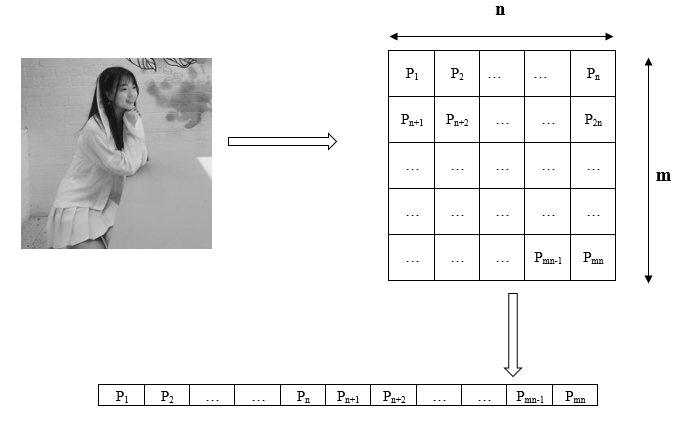
\includegraphics[width=\columnwidth]{image/Convert_image_as_one-dimension_matrix.png}
    \caption{Convert image as one-dimension matrix}
    \label{fig:figure}
   \end{figure}
   
   With the help of one-dimension matrix, \(P_{i}\) presents a specific pixel, which \(i\) is a sequence number of this carrier image. \(G(P_{i})\) means the gray level of this pixel, the value of \(G(P_{i})\) is an integer range from 0 to 255. \(M_{i}\) presents when converting watermarking message into binary, the ith binary value of this message. Hence, the value of \(M_{i}\) is 0 or 1. \(M_{i}\) and \(M_{i+1}\) are corresponding message bits respectively for \(P_{i} and P_{i+1}\). The next symbol is LSB(\(G(P_{i})\)), it stands for the value of last bit on this pixel. For example, the gray level of the 28th pixel is 125, LSB(\(G(P_{28})\)) is 1; the gray level of the 29th pixel is 126, LSB(\(G(P_{29})\)) is 0, etc. 
   
   Based on such definition, two adjacent pixels \(P_{i}\) and \(P_{i+1}\) are a LSB-pair pixels if they stratify (1) and (2): 
   
   \begin{equation}
   \\ G(P_{i}) = G(P_{i+1}) + 1 \quad or \quad G(P_{i}) = G(P_{i+1}) – 1
   \end{equation}
   \begin{equation}
   LSB(G(P_{i})) \neq M_{i} \quad and \quad LSB(G(P_{i+1})) \neq M_{i+1}
   \end{equation}
   
   We can use one sentence to conclude the definition: \textit{two adjacent pixels with adjacent gray levels and their LSB are different form corresponding message bits}.
   
   After filtering out the LSB pair, next question is to find out how the distortion changes when embedding the message. Due to each pixel of grayscale image occupies 8 bits, the distortion can be considered a list of 256 ordered elements. Each element represents the frequency of a specific gray level. The distortion list can be like:
   \[D = (d_{0}, d_{1}, d_{2} … , d_{253}, d_{254}, d_{255})\]
   For example, \(d_{35} = 47\) represents the total number of gray level 35 is 47. In order to calculate the distortion changes after watermarking, the original image distortion \(d_{1}\) and the watermarked image distortion \(d_{2}\) are required. The difference between \(d_{1}\) and \(d_{2}\): \(D’ = d_{2} - d_{1}\) is the distortion change which will be used in the latter evaluation. In this case: \(D’ = (d’_{0}, d’_{1}, d’_{2}…, d’_{253}, d’_{254}, d’_{255})\), \(d’35 = 47\) means the frequency of gray level 35 in watermarked image is 47 greater than original image. Therefore, if no message is embedded, all elements in \(D’\) should be 0.
   
   
   Two different situations when using LSB-pair method to embed message. First, suppose there have two pixels: \(G(P_{i}) = 124\), \(G(P_{i+1}) = 125\) and message bits: \(M_{i} = 1\), \(M_{i+1} = 0\). The LSB value of these two pixels can be obtained from calculation: \(LSB(G(P_{i})) = 0\), \(LSB(G(P_{i+1})) = 1\). Because these pixels meet requirement (1) and (2), these two pixels is a pair. Assuming the distortion change before doing LSB replacement is:
   \[D’_{before} = (…, d_{124} = a, d_{125} = b, …)\]
   Then embed the $i^{\text{th}}$ message bit into this image: \(G’(P_{i}) = 125\)
   \[D’_{after} = (…, d_{124} = a - 1, d_{125} = b + 1, …)\]
   Then embed the $(i+1)^{\text{th}}$ message bit into this image:\(G’(P_{i+1}) = 124\)
   
   \begin{align*} 
   D’_{after}  &= (…, d_{124} = a – 1 + 1, d_{125} = b + 1 - 1, …)\\
               &= (…, d_{124} = a, d_{125} = b, …)\\
               &= D’_{before}
   \end{align*}
   \[ \Rightarrow D’_{after} – D’_{before} = 0\]
   In this situation, the distortion is not change after embedding message.
   
   Another situation is when \(G(P_{i}) = 125\), \(G(P_{i+1}) = 126\), \(M_{i} = 0\), \(M_{i+1} = 1\). Assuming the distortion change before watermarking is \(D’_{before} = (…, d_{124} = a, d_{125} = b, d_{126} = c, d_{127} = d, …)\). Then using LSB replacement to embed message: 
   \[G’(P_{i}) = 124\] 
   \[G’(P_{i+1}) = 127\]
   \begin{multline*}
   D’_{after} = (…, d_{124} = a + 1, d_{125} = b - 1, \\
               d_{126} = c - 1, d_{127} = d + 1, …)
   \end{multline*}
   
   After that, calculating the distortion difference: 
   \begin{multline*}
   D’_{after} – D’_{before} = (|a + 1| - |a|) + (|b - 1| - |b|)\\
                   + (|c - 1| - |c|) + (|d + 1| - |d|)
   \end{multline*}
   According the definition, \(D’_{after} – D’_{before} < 0\) means after embedding message, the distortion of the image is reduced and vice versa. Assuming \(a > 0, b < 0, c < 0 \quad and \quad d > 0\), then we have:
   
   \begin{align*} 
   D’_{after} – D’_{before}    &= & &(|a + 1| - |a|) + (|b - 1| - |b|)\\
                               &  & &+ (|c - 1| - |c|) + (|d + 1| - |d|)\\
                               &= & &(a + 1 - a) + (1 – b + b) \\
                               &  & &+ (1 – c + c) + (d + 1 - d)\\
                               &= & &1 + 1+ 1+ 1\\
                               &= & &4 > 0
   \end{align*}
   
   However, when \(a + 1 < 0, b > 0, c > 0 \quad and \quad d + 1 < 0\)
   \begin{align*} 
   D_{after} - D_{before}  &= & &(|a + 1| - |a|) + (|b - 1| - |b|)\\
                           &  & &+(|c - 1| - |c|) + (|d + 1| - |d|)\\
                           &= & &( - 1 - a + a) + (b – 1 - b)\\
                           &  & &+ (c – 1 - c) + ( - 1 – d + d)\\
                           &= & &- 1 – 1 – 1 - 1\\
                           &= & &-4 < 0
   \end{align*}
   Except this is two specific situations. there still have varies of possible situations based on permutation and combination the value of a, b, c and d. However, in LSB-pair methods, it only interests in the value of D’after – D’before is positive or negative.  In other word, for this method, there is only two situations: distortion changes increasing or reducing. 
   
   In the situation of \(G(P_{i}) = 124\), \(G(P_{i+1}) = 125\), the distortion does not change. Because after embedding, we have: \(G’(P_{i}) = 125, G’(P_{i+1}) = 124\), the total number of gray level 124 and 125 does not change. It looks like these two pixels swap their position. It inspires a new way to handle the second situation. Since \(G(P_{i}) = 125, G(P_{i+1}) = 126, M_{i} = 0, M_{i+1} = 1\), if swap the position of two pixels before embedding, the result will be: \(G’(P_{i}) = 126, G’(P_{i+1}) = 125\). It is obvious that the distortion does not change after embedding. However, when doing regular LSB replacement for the second situation, the distortion change can be both positive and negative. Hence, the idea of LSB-pair is swapping pixels when the distortion change is positive and using regular LSB replacement when distortion change is negative. For instance, in the FIG. 2, if there has two pixels, \(G(P_{i}) = 125, G(P_{i+1}) = 126\), we do both LSB replacement and swap before doing LSB replacement directly. Then compare the distortion, keep the one with less distortion. 
   
   To sum up, this methods will check each to find out pixel pair which satisfies requirements (1) and (2). Then check the distortion change D’, if D’ is larger than 0, swap two pixels position. It can be concluded as following steps:
   \begin{enumerate}
   \item Check current pixel \(P_{i}\) and next pixel \(P_{i+1}\) is a pair or not. If not, go to step (5), otherwise, go to step (2).
   \item Calculate the distortion change for regular LSB replacement \(D'_{after} - D_{before}\), if it smaller than 0, go to step (3), otherwise, go to step (4)
   \item Swap two pixels position (value), then jump next iteration, go to one after next iteration.
   \item Do LSB replacement for this pixel \(P_{i}\) and next pixel \(P_{i+1}\), then jump next iteration, go to one after next iteration.
   \item Do LSB replacement for current pixel \(P_{i}\) than go to next iteration for next pixel.
   \end{enumerate}
   
   
   \begin{figure}[h]
   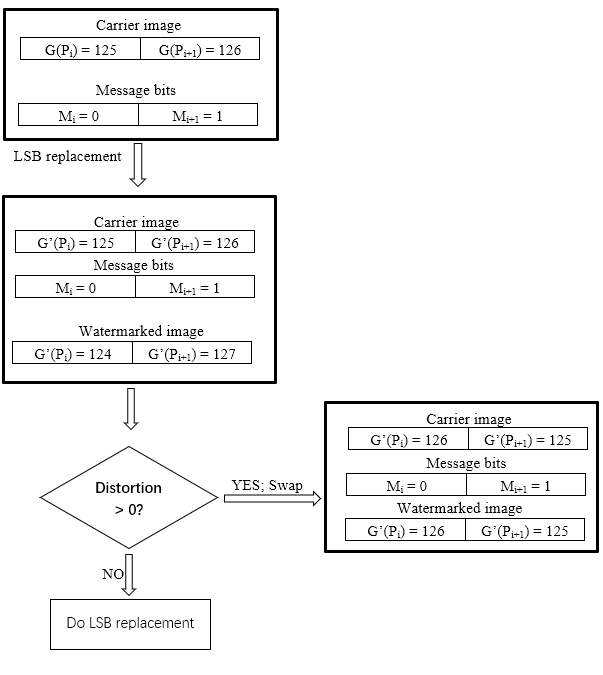
\includegraphics[width=\columnwidth]{image/LSB-pair_example.PNG}
   \caption{LSB-pair embedding}
   \label{fig:figure}
   \end{figure}
   
   \begin{figure}[h]
   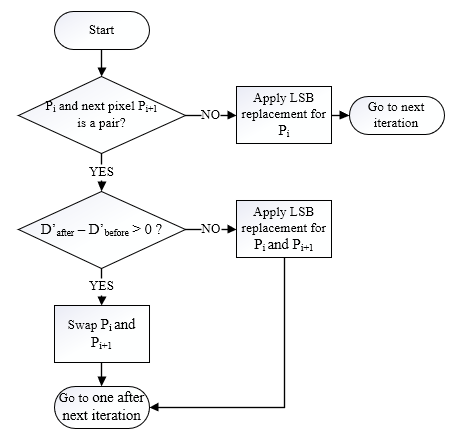
\includegraphics[width=\columnwidth]{image/processing_map.PNG}
   \caption{LSB-pair processing map}
   \label{fig:figure}
   \end{figure}
   
   
   \subsection{\label{sec:level2}LSB-triple-pair}
   
   Form our experiment for LSB-pair, 0.47\% of pixels meet requirement (1) and (2), 0.25\% of the pixels can do pixel position exchange to reduce the image distortion. For this situation, there is a demand that changing the condition of LSB-pair to expand its range of application.
   
   The LSB-triple-pair method is a modification of LSB-pair, in order to expend the LSB-pair the scope of application. In the previous method, each logic iteration considers two adjacent pixels \(P_{i} and P_{i+1}\) and their corresponding message bits Mi and Mi+1. In this method, three pixels are considered in each iteration: \(P_{i}, P_{i+1} and P_{i+2}\). The idea is, when the first and second pixel does not meet the condition (1) and (2) or distortion reduce requirements, this algorithm will try to find a pair between the first and third pixel to reduce the image distortion. The processing steps are:
   
   \begin{enumerate}
   \item Check current pixel \(P_{i}\) and next pixel \(P_{i+1}\) is a pair or not. If not, go to step (5), otherwise, go to step (2).
   \item Calculate the distortion change for regular LSB replacement \(D'_{after} - D_{before}\), if it is \textbf{greater than or equal to} 0, go to step (4), otherwise, go to step (3).
   \item Do LSB replacement for this pixel \(P_{i}\) and next pixel \(P_{i+1}\), then go one after next iteration.
   \item Check current pixel \(P_{i}\) and the one after next pixel \(P_{i+2}\) is a pair or not. If not, go to step (5), otherwise, go to step (6).
   \item Do LSB replacement for pixel \(P_{i}\), \(P_{i+1}\), \(P_{i+2}\) than jump two iterations, go to the fourth iteration.
   \item Calculate the distortion change for apply LSB replacement on these three pixels \((D’_{after} – D’_{before})\), if it lager than 0, go to step (7), otherwise, go to step (5).
   \item Swap the first and the third pixels position (value), do LSB replacement on the second pixel then jump next two iterations, go to the fourth iteration.
   \end{enumerate}
   
   For instance, there have three continuous pixels: \(G(P_{i}) = 125, G(P_{i+1}) = 124, G(P_{i+2}) = 126\), and their corresponding message bits: \(M_{i} = 0, M_{i+1} = 1 M_{i+2} = 1\). In this situation, first two pixels \(P_{i}\) and \(P_{i+1}\) meet the requirements (1) and (2). However, from the distortion definition, the distortion will not change after applying LSB replacement. Therefore, according to the algorithm, the value of these two pixels will not swap then the process will compare the first pixel with the third pixel. It is clear that \(P_{i}\) and \(P_{i+2}\) meet the requirements (1) and (2), assuming the distortion change will be greater than 0 after applying regular LSB replacement method, this method will swap \(P_{i} and P_{i+2}\) value then apply LSB replacement to these three pixels. FIG 4 shows the processing map.
   
   
   \begin{figure}[h]
   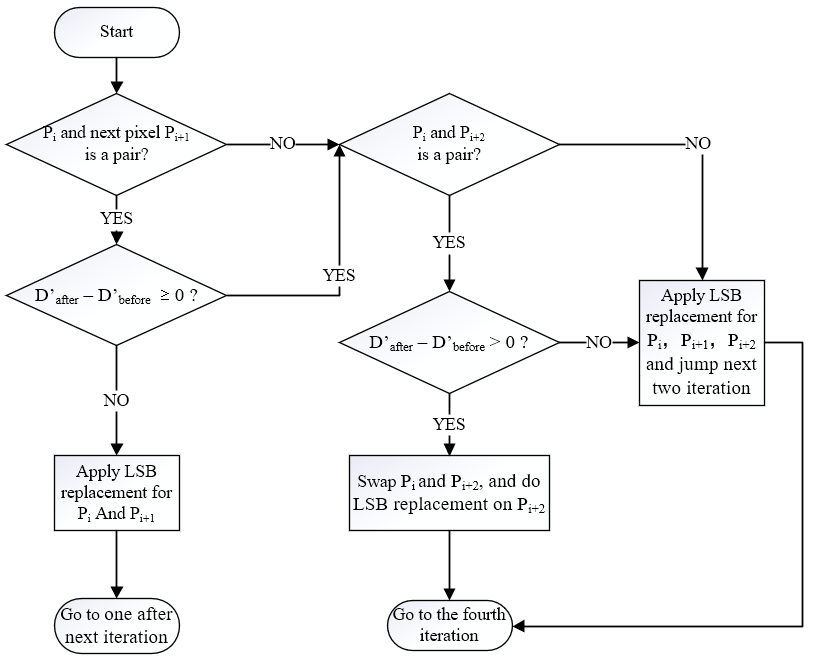
\includegraphics[width=\columnwidth]{image/processing_map_triple.PNG}
   \caption{LSB-triple-pair processing map}
   \label{fig:figure}
   \end{figure}    
   
   
   
   
   \subsection{\label{sec:level2}LSB-crossLine-pair}
   
   In this algorithm, it needs to change image sequence from one dimension back to two dimensions. FIG 5 shows that these methods it trying to find pixel pairs with next line pixel in the carrier image. For example, if the carrier image has n pixels horizontal and m pixels in vertical, this algorithm will try to find a pair between pixel \(P_{i} and P_{i+n}\). The idea of this method is also extending the application range of LSB-pair.  
   
   In this case, in order to avoid embedding system crush, the algorithm will stop LSB-crossline-pair detect and do LSB-pair only when moving to the pixel which is in last row. Because the embedding algorithm is from one pixel to another sequentially, when detected a crossline pair, it cannot jump the iteration of the next line’s pixel immediately. In code level, it needs an extra list to record the \(P_{i+n}\), if \(P_{i}\) and\(P_{i+n}\) meet all requirements of swapping value. Before each iteration, the code will check this list to see whether need to jump this iteration or not. However, in fact, this special situation cannot influence the result of LSB-crossline-pair detect. Because if \(P_{i}\) and \(P_{i+n}\) meet the conditions of value swap, the new \(P_{i+n}\) (pervious \(P_{i}\)) cannot satisfy requirement (2), which is \(LSB(G(P_{i+n})) \neq M_{i+n}\). In our experiments and coding, we skip this swapped pixel checking function, in order to save CPU process power and memory. However, logically, this makes no sense that check LSB-pair condition for an already swapped value pixel. This also can be an improved method for time-consuming and algorithm complexity for LSB-crossline-pair method. The basic processing steps are:
   
   \begin{enumerate}
   \item Check current pixel \(P_{i}\) is in the jump list or not. If yes, go to next iteration, otherwise, go to step (2).
   \item Check current pixel \(P_{i}\) and next pixel \(P_{i+1}\) is a pair or not. If not, go to step (5), otherwise, go to step (3).
   \item Calculate the distortion change for regular LSB replacement \((D’_{after} – D’_{before})\), if it \textbf{greater than or equal to} 0, go to step (5), otherwise, go to step (4)
   \item Do LSB replacement for this pixel \(P_{i}\) and next pixel \(P_{i+1}\), then go next iteration.
   \item Check current pixel \(P_{i}\) and the one after next pixel \(P_{i+n}\)n is a pair or not. If not, go to step (6), otherwise, go to step (7).
   \item Do LSB replacement for pixel \(P_{i}, P_{i+1}, P_{i+n}\) , record \(P_{i+n}\) into jump list then jump next iterations, go to the third iteration.
   \item Calculate the distortion change for apply LSB replacement on these three pixels \((D’_{after} – D’_{before})\), if it greater than 0, go to step (8), otherwise, go to step (6).
   \item Swap \(P_{i}\), and the \(P_{i+n}\) position (value), do LSB replacement on \(P_{i+1}\) then record \(P_{i+n}\) into jump list, after that, jump next iteration, go to the third iteration.
   \end{enumerate}
   
   For instance, there have three continuous pixels: \(G(P_{i}) = 125, G(P_{i+1}) = 124, G(P_{i+n}) = 126\), and their corresponding message bits: \(M_{i} = 0, M_{i+1} = 1 M_{i+n} = 1\). In this situation, first two pixels \(P_{i} and P_{i+1}\) meet the requirements (1) and (2). However, from the distortion definition, the distortion will not change after applying LSB replacement. Therefore, according to the algorithm, the value of these two pixels will not swap then the process will compare the first pixel with the next line pixel \(P_{i+n}\). It is clear that \(P_{i}\) and \(P_{i+n}\) meet the requirements (1) and (2), assuming the distortion change will be greater than 0 after applying regular LSB replacement method, this method will swap \(P_{i} and P_{i+n}\) value then record \(P_{i+n}\). After that, applying LSB replacement to these three pixels.
   
   \begin{figure}[h]
   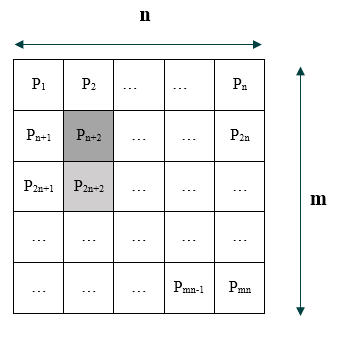
\includegraphics[width=\columnwidth]{image/LSB-crossline-pair.PNG}
   \caption{LSB-crossline-pair}
   \label{fig:figure}
   \end{figure}   
   
   
   
   
   \subsection{\label{sec:level2}Combination}
   
   The method LSB-crossline-pair and LSB-triple-pair both can improve the performance. Theoretically, combining these two functions into one might have a better performance than both, this combination method is named as LSB-combine-pair. Based on comparing the performance of LSB-crossline-pair and LSB-triple-pair, the LSB-crossline-pair have better performance and more stability in reducing image distortion than LSB-triple-pair. Hence, the idea of the new approach is using LSB pair method at first, if these pixels are not a pair, try to find LSB-crossline-pair. If these pixels still not meet the requirement of distortion reduce, then try to find a pair using LSB-triple-pair. A detailed discusses and analyses the performance of these two methods will be covered in next part. FIG 6 shows a simplification processing map is:
   
   \begin{figure}[h]
   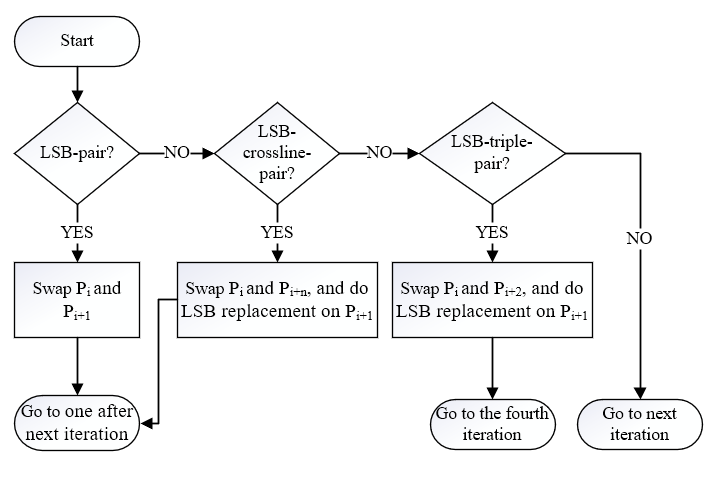
\includegraphics[width=\columnwidth]{image/processing_map_ultra.PNG}
   \caption{LSB-combine-pair processing map}
   \label{fig:figure}
   \end{figure}   
   
   
   
       
   \section{\label{sec:level1}Evaluation}
   
   Before comparing the performance of these methods, one thing need to be mentioned is that the error rate of extracting watermarking message using these methods is 0\% of these 10,000 image sets. The robustness is one of the core features of digital watermarking. The experiments show that these methods are stable and reliable enough to be considered as new methods in digital watermarking field.
   
   PSNR, Hae, SSIM are three measurement approaches for evaluating image quality. Ten thousand images from GHIM-10K \cite{liu2015content} have been used in this experiment. All images are grayscale images which in 400*300 or 300*400 resolution. A message with 6,219 characters in ASCII code which is 6,219 bytes size has been embedded into these grayscale image. This experiment has tested five LSB embed methods, including original LSB replacement, LSB-pair, LSB-crossline-pair, LSB-triple-pair and LSB-combine-pair. 
   
   
   \subsection{\label{sec:level2}Hae}
   
   Histogram absolute error (Hae) is a method which intuitively indicates the total difference between original image and watermarked image. In the previous part we had defined the distortion distribution of gray level pixels is: \(D = (d_{0}, d_{1}, d_{2} … , d_{253}, d_{254}, d_{255})\); the distortion changes between watermarked image and original image is: \(D' = D_{2} - D_{1}, D' = (d'_{0}, d'_{1}, d'_{2} … , d'_{253}, d'_{254}, d'_{255})\). Yang \cite{ren2014image} used a formula to calculate histogram absolute error:
   $$h(n) = \sum_{i=1}^{H}*\sum_{j=1}^{W}(\delta(n,P(i,j)))$$
   
   where
   $$\delta(u,v) = \begin{cases} 1, & u = v \\ 
   0, & u \neq v \end{cases}$$
   
   In his formula, H and W is the height and width of the carrier image respectively. P(i,j) is the pixel value, in this report, it is the same as \(G(P_{i})\) which refer to the gray level of this pixel. n represents the gray intensity value, in an 8 bits per pixel image, \(n \in [0,255]\) and \(n\in N\). In previous image distortion definition, this formula can transform to:
   $$h(n) = \sum_{i=1}^{255} d_{i}$$
   
   Then calculate distortion change:
   $$Hae = \sum_{i=1}^{255} (d2_{i} - d1_{i}) = \sum_{i=1}^{255} d'_{i}$$
   
   Form the definition, Hae smaller than 0 represents distortion reduce, vise verse. FIG 7 shows the pseudocode of this method.
   
   \begin{figure}[h]
   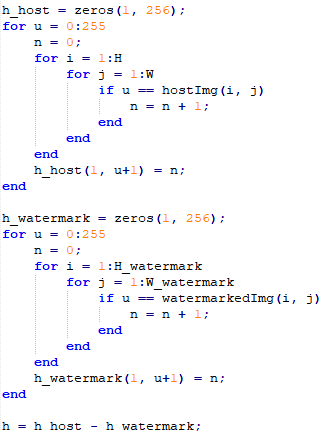
\includegraphics[width=\columnwidth]{image/Pseudocode_Hae.PNG}
   \caption{Pseudocode of Hae}
   \label{fig:figure}
   \end{figure}   
   
   
   
   \subsection{\label{sec:level2}PSNR}
   
   Peak signal-to-noise ratio (PSNR) is one of the important and commonly used measurements to evaluation image changes. PSNR is an engineering term for the ratio between the maximum possible power of a signal and the power of corrupting noise that affects the fidelity of its representation. Higher the value of MES represents higher the error and worse picture quality. \cite{eratne2009fast}
   
   The formula of PSNR is:
   
   \begin{align*}  
   PSNR    &=  10* \log_{10} \frac{MAX^2_{1}}{MSE} \\
           &=  20 *\log_{10} \frac{MAX_{1}}{\sqrt{MSE}}
   \end{align*} 
   MSE is mean squared error, the formula of MSE is:
   
   $$MSE = \frac{1}{mn}\sum_{i=0}^{m-1}\sum_{j=0}^{n-1} [I(i,j)-K(i,j)]^2$$
   
   The MAX means the maximum possible value of the image. For example, if there is a picture which is 8 bits per pixel, the maximum value is 255, 14 bits is 16383. As for colorful picture, there has three MSE value corresponding Red, Green and Blue, and get three PSNR for each color as well. Which means, a colorful image has a vector of three PSNR value to evaluate its quality.
   
   
   Generally, 30 to 50 dB for 8 bits picture, 60 to 80 dB for 16bits picture is considered as an acceptable image. However, PSNR is not friendly for human vision. The value of PSNR is not exactly how we humans think. Because it just uses mean square value to evaluate image, does not consider the image inside, which means, it does not care about what this image is, just evaluate the total and average value or energy changes.
   
   Human vision can be different for different individual. It is a very complex and cannot treat as a liner system. We still have limited knowledge about it. The result of human vision evaluation can be influenced by individual’s background, knowledge and motivation. The observation environment also is a significant parameter. [some cites here] FIG 8 is an example, XXXXXX used in his paper. The middle image is the original image, it is obviously that most people think the left one is more similar than right one. However, these two have the same PSNR value. For this reason, our experiment only uses PSNR as a reference measurement, not a core indicator for image changes.
   
   \begin{figure}[h]
   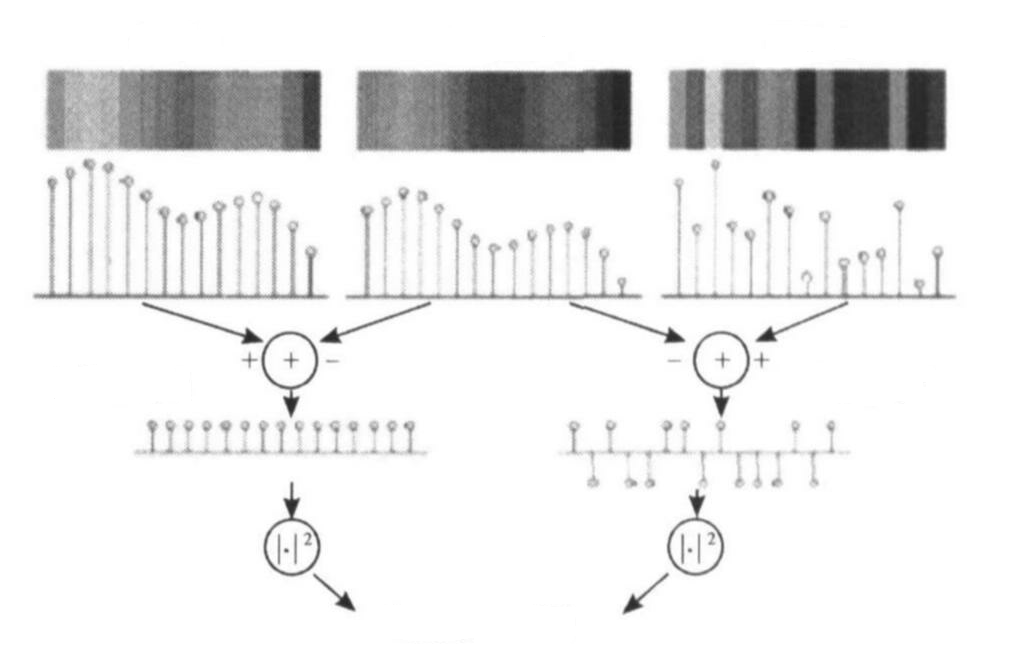
\includegraphics[width=\columnwidth]{image/PSNR_example.png}
   \caption{Pseudocode of Hae}
   \label{fig:figure}
   \end{figure} 
   
   
   \subsection{\label{sec:level2}SSIM}
   
   Structural similarity index measure (SSIM) performance well for static image measure. Regular approaches are going to solve absolute errors, however, SSIM is perception-based model which can consider image degradation. [some cites here] Image degradation is considered as a perceived change in the structural information of the image. It not only considers about RGB color but also YUV. This approach believes each pixel have strong inter-dependencies especially when they are spatially close.
   
   According to Wang’s research, SSIM has better performance than PSNR. However, it cannot totally solve the problem which PSNR has. \cite{wang2005structural} The algorithm for SSIM is complex, generally, it separates image to various windows and measure between windows. The formula is:
   
   \[SSIM ( f ,g ) = l ( f ,g )c ( f ,g )s ( f ,g )\]
   $$\begin{cases} l(f,g) = \frac{2\mu_{f}\mu_{g} + C_{1}}{\mu^2_{f} + \mu^2_{g} + C_{1}}\\ 
   c(f,g) = \frac{2\sigma_{f}\sigma_{g} + C_{2}}{\sigma^2_{f} + \sigma^2_{g} + C_{2}}\\
   s(f,g) = \frac{\sigma_{fg} + C_{3}}{\sigma_{f}\sigma_{g} + C_{3}}
   \end{cases}$$
   
   The first term is the luminance comparison function which measures the closeness of the two images’ mean luminance \((\mu_{f}\)  and \(\mu_{g})\). c(f,g) is the function of measure contrast comparison, and the third item is for the structure comparison. \(C_{1}\), \(C_{2}\) and \(C_{3}\) is positive constants which are used to provide from null denominator.
   
   
   \subsection{\label{sec:level2}Experiment and results}
   
   This part discusses the performance of four kinds of LSB-pair methods using ten thousand image set. FIG 8 is the digital watermarking image which embedded information invisibly, (a) is the original 512*512 carrier image. (b), (c), (d), (e), (f) is done by original LSB replacement, LSB-pair, LSB-crossline-pair, LSB-triple-pair, LSB-combine-pair respectively. 
   
   
   \begin{figure}[h]
   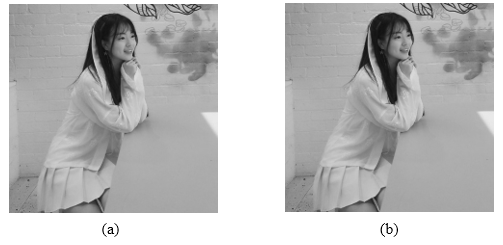
\includegraphics[width=\columnwidth]{image/ab.PNG}
   \label{fig:figure}
   \end{figure} 
   
   \begin{figure}[h]
   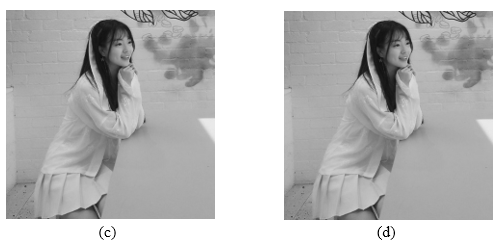
\includegraphics[width=\columnwidth]{image/cd.PNG}
   \label{fig:figure}
   \end{figure} 
   
   \begin{figure}[h]
   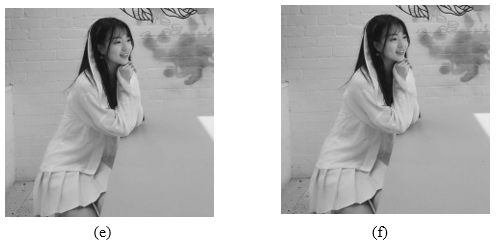
\includegraphics[width=\columnwidth]{image/ef.PNG}
   \caption{Watermarking embedding}
   \label{fig:figure}
   \end{figure} 
   
   FIG 9 shows the PSNR for regular LSB replacement, LSB-pair, LSB-crossline-pair, LSB-triple-pair and LSB-combine-pair. It is clear that all these methods have the same PSNR value. The prove of original LSB replacement and LSB-pair having same PSNR value is: 
   
   \begin{itemize}
     \item If two adjacent pixels are not a pair, they need to be applied for original LSB replacement, hence, the PSNR not change when two pixels are not a pair.
     \item Assuming \(P_{i}, P_{i+1}\) meets LSB pair requirements, \(P_{i} = P_{i+1} + 1\) and \(LSB(P_{i}) = 0\), form the definition, we have \(M_{i} = 1, M_{i+1} = 0\).
     \item If use original LSB replacement, the embedded \(P'_{i} = P_{i + 1}\), \(P'_{i+1} = P_{i+1} – 1\), \(LSB(P_{i}) = 1, LSB(P_{i}) = 0\). In this case, calculate MSE difference for these two pixels: \((P'_{i} - P_{i})^2 + (P'_{i+1} - P_{i+1})^2 = 1 + 1 = 2\)
     \item If use LSB-pair, swap Pi and Pi+1 at first, get \(P'-{i} = P_{i+1} = P_{i} - 1, P'_{i+1} = P_{i} = P_{i+1} + 1\). In this case, calculate MSE difference for these two pixels: \((P'_{i} - P_{i})^2 + (P'_{i+1} - P_{i+1})^2 = 1 + 1 = 2\). Therefore, the PSNR does not change compare with using original LSB replacement.
     \item The same derivation process for the situation \(P_{i} = P_{i+1} – 1\).
   \end{itemize}
   
         
   To sum up, this proves can be extended to other LSB-pair variations methods, original LSB replacement method and LSB-pair with its variations have the same value in PSNR. Due to this phenomenon, PSNR cannot be a measurement method in this situation. However, it can be a verification method to validate the LSB-pair method is applied correctly or not.
   
   
   Table 1 shows the average, maximum and minimum PSNR value in this image set. Form the PSRN definition, 1 to 5 dB change is an acceptable image change.
   
   \begin{table*}
   \begin{tabular}{ |c|c|c|c|  }
    \hline
    \multicolumn{4}{|c|}{PSNR(dB)} \\
    \hline
    LSB methods        &Mean           &Maximum        &Minimum\\
    \hline
    LSB                &1.743856156    &4.247659738    &0.33989157\\
    \hline
    LSB-pair           &1.743856156	&4.247659738	&0.33989157\\
    \hline
    LSB-crossline-pair &1.743856156    &4.247659738    &0.33989157\\
    \hline
    LSB-triple-pair    &1.743856156    &4.247659738    &0.33989157\\
    \hline
    LSB-combine-pair   &1.743856156    &4.247659738    &0.33989157\\
    \hline
   \end{tabular}
    \caption{Summary of PSNR}
   \end{table*}
   
   \begin{figure}[h]
   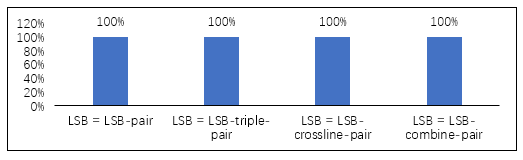
\includegraphics[width=\columnwidth]{image/PSNR.PNG}
   \caption{PSNR result}
   \label{fig:figure}
   \end{figure} 
   
   
   FIG 11 shows the experiment result for Hae. This method calculates the total difference between original image and watermarked image. If it is lower than 0, it means the distortion is smaller. Comparing original LSB replacement with others, average 6\% images have lower distortion than other four LSB-pair methods, LSB-pair takes the lowest (5.18\%) and LSB-combine-pair is the highest (6.96\%). As for higher distortion, LSB-pair performance worst, original LSB replacement has 24.53\% of images higher than LSB-pair. LSB-combine-pair performance the best, 31.28\% have low distortion than original LSB replacement. However, the most number of image sets have the same distortion, they occupy about 60-70\%. 
   
   As for comparing LSB-pair and its variations in Hae, the result generally looks the same – about 70\% data set have the same distortion value. Nonetheless, when put attention on the detail, the features of each method are all different. Advanced LSB-pair methods (LSB-crossline-pair, LSB-triple-pair, LSB-combine-pair) all have a higher percentage in reducing distortion than increase distortion. LSB-crossline-pair performance better than LSB-triple-pair: 18.03\% have lower distortion than LSB-triple-pair and 9.96\% higher distortion, the rest images have the same distortion. This is the main reason that in LSB-combine-pair, crossline pair detect have higher priority than jump pixel detect. As for LSB-combine-pair, it performs better than others.
   
   Table 2 shows the summary of Hae. It indicates that Hae of original LSB replacement is 0.0224\%, 0.0642\%, 0.0504\%, 0.0834\% higher than LSB-pair, LSB-crossline-pair, LSB-triple-pair, LSB-combine-pair respectively on average. One interesting thing is the maximum of Hae is the same. When sourcing back, the images which cause these outlier values are the same one. In this image, it has three unusual features: over 70\% pixels are in the same color (gray level: 0); pixel gravy level changes sharply; there does not have any LSB pair which can be detected. By above finds, can get conclude that: the carrier image best has complex compositions and variety of colors.   
   
   \begin{figure}[h]
   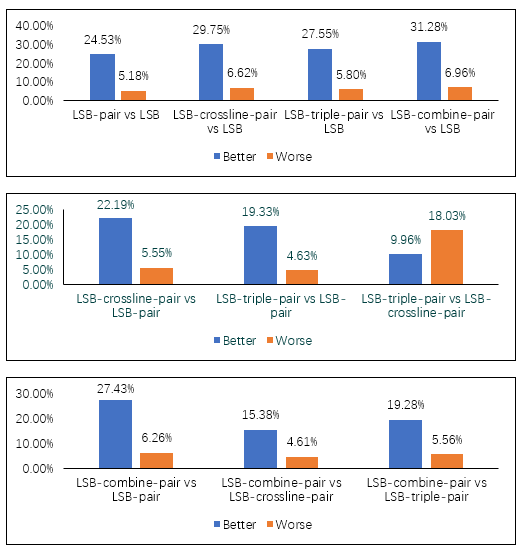
\includegraphics[width=\columnwidth]{image/Hae.PNG}
   \caption{Hae result}
   \label{fig:figure}
   \end{figure} 
   
   
   \begin{table*}
   \begin{tabular}{ |c|c|c|c|c|c|c|  }
    \hline
    \multicolumn{7}{|c|}{Histogram absolute error} \\
    \hline
    LSB methods    &Minimum&1st Quartile	&Median	&Mean	&3rd Quartile	&Maximum\\
    \hline
    LSB&               16950	&42280	&42868	&43693.44	&43534	&110376\\
    \hline
    LSB-pair	        &16722	&42274	&42862	&43683.64	&43526	&110376\\
    \hline
    LSB-crossline-pair	&16398	&42262	&42855	&43665.42	&43512	&110376\\
    \hline
    LSB-triple-pair	&16428	&42268	&42858	&43671.42	&43518	&110376\\
    \hline
    LSB-combine-pair	&15832	&42254	&42851	&43657.03	&43506	&110376\\
    \hline
   \end{tabular}
    \caption{Summary of Hae}
   \end{table*}
   
   
   FIG 12 and table 3 pints the value of SSIM. Due to SSIM difference is tinny, we use (1 - SSIM) * 10000 to zoom in the difference, in this case, the lower value in the table, the better performance in SSIM it has. Generally, all these advanced LSB-pair methods have poorer performance than original LSB replacement. Besides original LSB replacement methods, LSB-triple-pair has the best performance, 17.19\% of the watermarked images are better than which applying original LSB-replacement; for LSB-pair, this rate 10.78; 9.81\% for LSB-crossline-pair; 11.56\% for LSB-combine-pair. When comparing with LSB-triple-pair with LSB-crossline-pair and LSB-combine-pair, 64.94\% and 89.96\% of images have better SSIM value. One thing needs to be pay attention is, LSB-triple-pair performance better than LSB-pair when comparing with original LSB replacement. However, only 25.55\% of images have better SSIM than LSB-pair. It means, if one image has worse performance in LSB -pair than original LSB replacement, it has a high possibility that performance worse in LSB-triple-pair than original LSB replacement, vice versa. LSB-combine-pair is the worst in this evaluation, but that not means that LSB-combine-pair is not a suitable digital watermarking embedding method, table 3 points it has narrow gaps with others. 
   
   \begin{figure}[h]
   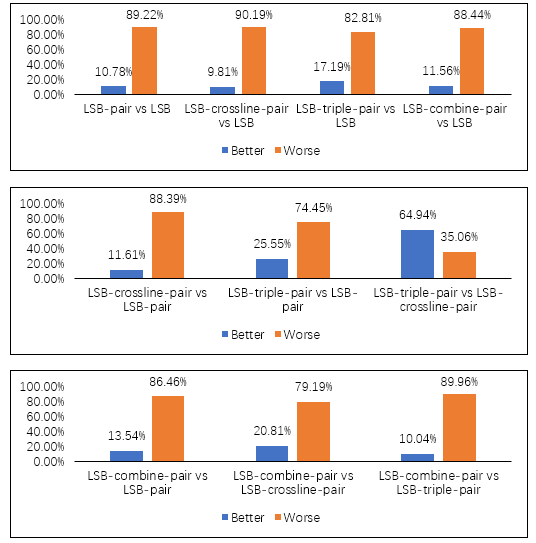
\includegraphics[width=\columnwidth]{image/SSIM.PNG}
   \caption{SSIM result}
   \label{fig:figure}
   \end{figure} 
   
   
   \begin{table*}
   \begin{tabular}{ |c|c|c|c|c|c|c|  }
    \hline
    \multicolumn{7}{|c|}{(1 - SSIM) * 10000} \\
    \hline
    LSB methods    &Minimum&1st Quartile	&Median	&Mean	&3rd Quartile	&Maximum\\
    \hline
    LSB	            &28.82922	&28.82922	&2.270463	&28.82922	&2.270463	&2.270463\\
    \hline
    LSB-pair	        &28.84012	&28.84012	&2.270217	&28.84012	&2.270217	&2.270217\\
    \hline
    LSB-crossline-pair	&28.87481	&28.87481	&2.27009	&28.87481	&2.27009	&2.27009\\
    \hline
    LSB-triple-pair	&28.8617	&28.8617	&2.270335	&28.8617	&2.270335	&2.270335\\
    \hline
    LSB-combine-pair	&28.89619	&28.89619	&2.270018	&28.89619	&2.270018	&2.270018\\
    \hline
   \end{tabular}
    \caption{Summary of SSIM}
   \end{table*}
   
   
   There are no precise rules for selecting the Hae, PSNR or SSIM when the evaluation of image quality is required. The aim of this methods is to reduce the distortion changes, therefore, the result of Hae is considered as the highest priority. PSNR and SSIM are considered as assist evaluation approaches also need to be attention which can guarantee the image quality after embedding message. 
   
   In theoretical, LSB-crossline-pair has less chances to find pairs than LSB-triple-pair. Because in a n*m image, except last two pixels, LSB-triple-pair has \(n*m -2\) chances to find a pair. However, LSB-crossline-pair only has \(n*m – n\) chances, except the pixels last row. Therefore, if the image is as large enough, the method LSB-triple-pair should perform \(1/m\) better than LSB-crossline-pair, due to it has 1/m more chances to find pairs theoretically. However, the experiment results show that LSB-crossline-pair has better performance in Hae which is against the theory. 
   
   For the pixel distance, assuming start with pixel \(P_{7}\), LSB-pair compares with \(P_{8}\) which has 1 Euclidean distance; LSB-crossline-pair compares with \(P_{8}\) and \(P_{12}\) with also has 1 Euclidean distance; LSB-triple-pair compares with \(P_{8}\) and \(P_{9}\) which has 1 to Euclidean distance. According to LSB-crossline-pair has better performance in reducing distortion then LSB-triple-pair, we can make a prediction that the lower Euclidean distance will have better performance in LSB-pair serious methods. Therefore, we can predict LSB-diagonal-pair (\(P_{7}\) with \(P_{13}\)) has better performance than LSB-crossDoubleLine-pair (\(P_{7}\) with \(P_{17}\)).
   [Result for LSB-diagonal-pair and LSB-crossDoubleLine-pair to proving this assumption]
   
   
   \begin{figure}[h]
   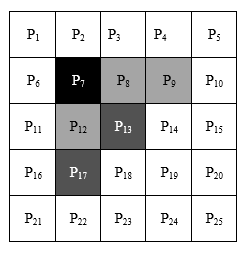
\includegraphics[width=\columnwidth]{image/Euclidean_distance.PNG}
   \caption{Euclidean distance}
   \label{fig:figure}
   \end{figure} 
   
   
   
   
   
   \section{\label{sec:level1}Conclusion and Future Work}
   
   In this paper, a comparison has been made using the PSNR, Hae and SSIM at different LSB-pair embedding methods. The result shows that the LSB-pair methods can reduce image distortion and within the SSIM permit, combine multiple LSB-pair methods can reduce distortion effectively. The performance of distortion reducing have negative correlation with Euclidean distance for pixel pair.
   
   Future work includes extending these methods for color image which need to consider three vectors (RGB) instead of one (gray). Besides crossline and jump one-pixel pair. Another work is that find a balanced Euclidean distance for advanced LSB-pair methods between SSIM and distortion.  
   
   
   
   \section{\label{sec:level1}Acknowledgment}
   
   The author would like to thank the reader and anyone who reviewed this paper and gave suggestions, which improved the quality of this paper. The author would also like to thank Winnie who provide grayscale images for test and experiments. 
   
   
   
   
   \bibliographystyle{plain}
   \bibliography{references}
   \end{document}
   
   